\documentclass[conference]{IEEEtran}
\IEEEoverridecommandlockouts
\emergencystretch=1em
\usepackage{cite,amsmath,graphicx,booktabs,url,balance}
\def\BibTeX{{\rm B\kern-.05em{\sc i\kern-.025em b}\kern-.08em T\kern-.1667em\lower.7ex\hbox{E}\kern-.125emX}}
\begin{document}

\title{Confusable Telecom APIs: When Retrieval Succeeds\\but Tool Selection Fails}

\author{\IEEEauthorblockN{Vineeth Reddy Vallapureddy}
\IEEEauthorblockA{\textit{Independent} \\ 0708vineeth@gmail.com}
\and
\IEEEauthorblockN{Alekhya Katukuri}
\IEEEauthorblockA{\textit{Independent} \\ alekhyahy9@gmail.com}
\and
\IEEEauthorblockN{Satya Sai Prudhvi Krishna Nikku}
\IEEEauthorblockA{\textit{Independent} \\ prudhvinikku@gmail.com}}

\maketitle

\begin{abstract}
Telecom management APIs are generated from shared information models, so a
single operator stack exposes hundreds of operations whose names differ by one
token while their effects differ completely. We harvest 1,062 tool
definitions from 79 published TM~Forum Open API specifications and label
confusability from the specifications alone, independently of any retriever:
54.8\,\% of the catalogue has a sibling operation sharing its verb and
most of its entity tokens. On 419 operator requests we compare full-schema
prompting, dense and lexical retrieval, PA-Tool-style renaming, and a
LoRA-tuned 1.7B router that sees no schemas at all. In a controlled within-query injection, confusers displace the gold tool from
rank one ($-11.3$ points) but rarely out of the top five ($-2.8$): the failure
moves from retrieval to discrimination, and the selector amplifies it,
converting 95.7\,\% of retrieved distinct tools into correct answers against
80.3\,\% of confusable ones. At $N=200$ full-schema prompting is no better than top-5 retrieval on
confusable tools (58.4 both) despite 21$\times$ the tokens. Renaming does not help: the standards code is the disambiguator.
The router's accuracy is invariant to catalogue size where retrieval's is not,
and the two are complementary: their union gains 8.1 points at 1,062 tools,
9.4 of them on confusable tools.
Abstention is the weakest link: with the correct tool absent, the pipeline
still names one 71\,\% of the time, worse when siblings are present.

\end{abstract}

\begin{IEEEkeywords}
LLM agents, tool selection, telecom management APIs, retrieval, small language models
\end{IEEEkeywords}

\section{Introduction}
Agentic assistants for network and service operations are converging on the
same interface: the model is handed a set of tool (API) schemas and must pick
one and fill its arguments. In telecom this tool set is not small. A single
operator stack exposes order management, service and resource inventory,
catalogue, assurance, activation and billing interfaces, each with dozens of
operations. Published work has established that selection accuracy falls as the
tool set grows and that retrieving a small candidate set before prompting
recovers most of the loss~\cite{ragmcp,toollery}. It has also
established that a small model can internalise a \emph{fixed} tool catalogue by
fine-tuning, removing schemas from the prompt
entirely~\cite{qlora_tools}, and, in the opposite direction, that much of
what looks like a capability gap is really schema-name misalignment that can be
fixed by renaming tools rather than retraining them~\cite{patool}.

What is missing is a measurement of these choices on a tool catalogue that
telecom actually has. Existing telecom agent benchmarks evaluate
troubleshooting and dialogue over small, curated tool sets~\cite{telcoagent,ctbench,wirelessbench};
generic tool-routing studies use large but semantically scattered catalogues
where a nearest-neighbour lookup is usually enough. Standardised telecom
management APIs are different in a specific way: they are generated from a
common information model, so the same operation verb is applied to entities
whose names differ by one token. \texttt{listServiceCatalog},
\texttt{listResourceCatalog}, \texttt{listEntityCatalog} and
\texttt{listProductCatalog} are four different APIs, four different endpoints
and four different operational meanings, expressed in almost the same words.
We call such tools \emph{confusable}, and we show they are the majority case,
not a corner case.

To our knowledge this is the first tool-routing study on a standardised
telecom management catalogue at this scale. This work-in-progress paper makes
three contributions.
\textbf{(i)} We build a tool catalogue of 1,062 operations harvested from
79 published TM~Forum Open API specifications~\cite{tmforum}, and define a
confusability label that is computed from the specifications alone and is
independent of any retriever: 54.8\,\% of the catalogue is confusable.
\textbf{(ii)} We evaluate full-schema prompting, dense and lexical retrieval,
PA-Tool-style renaming, and a LoRA-tuned description-free 1.7B router on the
same queries, and report accuracy separately for confusable and distinct tools.
\textbf{(iii)} Because a wrong tool in this domain is not uniformly wrong, we
report a severity-weighted error cost and a destructive-misfire rate alongside
accuracy, and we score argument generation separately from selection so the two
failure modes do not mask each other.


\section{Related Work}
Retrieving a small candidate set before prompting is the established answer to
catalogue growth~\cite{ragmcp,toollery}, so full-schema prompting is a
historical baseline and dense retrieval the method to beat. Conversely, tool
knowledge can be internalised by fine-tuning so the prompt carries no schemas,
shown on an industrial asset-operations catalogue~\cite{qlora_tools}; and
substituting a retriever for a router model is reported to preserve selection
but not abstention~\cite{ondevice_routing}. PA-Tool argues no training is
needed, since small-model tool errors are dominated by schema names that do not
match pretraining~\cite{patool}. We include all three positions. Telecom agent
benchmarks evaluate troubleshooting over small curated tool
sets~\cite{telcoagent,ctbench}, and WirelessBench argues for tolerance-aware
scoring because flat accuracy hides catastrophic errors~\cite{wirelessbench};
we adopt that argument for routing, on a far larger catalogue.


\section{A Real Telecom Tool Catalogue}
\subsection{Harvesting}
We cloned the published OpenAPI/Swagger documents of the TM~Forum Open API
suite~\cite{tmforum} and flattened every \texttt{operationId} into one tool,
keeping its HTTP method, path, summary, description and parameter list. This
yields 1,891 operations. We then remove notification plumbing
(\texttt{/listener/*} callbacks and \texttt{/hub} subscription endpoints),
which is
mechanically duplicated across every API and would inflate both the catalogue
size and the confusability rate. The resulting catalogue has \textbf{1,062
tools over 79 APIs}: 497 reads, 386 state-changing (POST/PUT/PATCH) and
179 destructive (\texttt{DELETE}) operations.

\subsection{Confusability}
Labelling confusability with an embedding model would make the label a function
of the system under test. We therefore define it on the specifications only.
Two tools $a,b$ are confusable if they share an HTTP method and an operation
verb, belong to \emph{different} APIs, and their entity-token sets satisfy
$J(a,b)=|E_a\cap E_b|/|E_a\cup E_b|\ge 0.5$, where $E$ is the camel-case split
of the \texttt{operationId} with the leading verb removed. A tool is confusable
if at least one such partner exists. By this rule \textbf{582 of
1,062 tools (54.8\,\%)} are confusable: the phenomenon is native
to the standard, not constructed for the experiment. One representative family: \texttt{TMF620\_\allowbreak listCatalog} (product catalogue),
\texttt{TMF633\_\allowbreak listServiceCatalog}, \texttt{TMF634\_\allowbreak listResourceCatalog},
\texttt{TMF662\_\allowbreak listEntityCatalog} and \texttt{TMF909\_\allowbreak listServiceCatalog}
are five distinct endpoints in five distinct APIs.



\subsection{Queries}
For a stratified sample over (confusable $\times$ severity), capped at four
tools per API, a local instruction model writes one operator utterance per
tool from the API title, summary and required parameters. Automated gates
reject any utterance leaking the \texttt{operationId}, naming a domain owned
by a different API, or naming its own API title or TMF code. This yields
\textbf{419 queries} with a gold tool and gold arguments.


\section{Experimental Setup}
Everything runs locally on an Apple M4~Pro (24\,GB), so costs are tokens and
latency, not prices. The selector is Qwen3.5 (8B class, 4-bit, ollama) with
reasoning disabled; the router is Qwen3-1.7B~\cite{qwen3} (bf16, MLX)\@.
Retrieval uses \texttt{nomic-embed-text}~\cite{nomic} and BM25 over one
document per tool (name, method, path, API title, summary, parameters).
Greedy decoding throughout.

\textbf{Catalogue sizes.} For a query with gold tool $g$, the catalogue of
size $N$ is $g$ plus $N-1$ distractors drawn deterministically with a per-query
seed. Confusability is re-evaluated \emph{within} that subset: a trial is
confusable if at least one confuser of $g$ is present.

\textbf{Methods.} \texttt{full} places all $N$ schemas in the prompt;
\texttt{dense5}/\texttt{bm25\_5} prompt with five retrieved candidates;
\texttt{*\_rename} replaces \texttt{TMF633\_\allowbreak listServiceCatalog} with a
pretraining-aligned \texttt{list\_service\_catalog}~\cite{patool};
\texttt{direct} supplies no schemas. The routers are the 1.7B prompted
description-free, the tuned one LoRA-adapted (rank 8, lr $10^{-4}$, 1,500
steps) on 11,390 \emph{template-generated} pairs covering all 1,062 tools, with no model-written utterances, so the evaluation queries are out of distribution
for the router by construction. \texttt{hybrid} is the union of the tuned
router's single prediction with the dense top-5, scored by the same selector.

\textbf{Metrics.} Top-1 accuracy, split confusable/distinct; candidate recall;
severity-weighted error cost $c_{\mathrm{sev}}$ (a wrong answer costs 1, 3 or
10 according to whether the \emph{chosen} tool is a read, a state-changing
operation or a \texttt{DELETE}; a correct answer costs 0); mean prompt tokens and wall-clock.
Abstention is a separate condition in which the gold tool is removed and
\texttt{NONE} is the only correct answer. Argument generation is scored in a
second stage conditioned on the gold tool, so a parameter error is never
charged to the router.


\section{Results}
\subsection{Retrieval degrades steeply, and unevenly}
Retrieval recall, measured with no language model in the loop, degrades steeply. Dense top-1 recall falls from
79.7\,\% at 25 tools to 32.5\,\% at the full catalogue of 1,062; top-5
recall falls from 97.4\,\% to 61.1\,\%. BM25 behaves similarly overall
(27.7\,\% / 60.1\,\% at full scale) but is far more sensitive to
confusability: at full scale its top-5 recall is 77.3\,\% on distinct tools and
43.4\,\% on confusable ones, a 33.9-point gap, against a 12.9-point gap for
dense retrieval. Lexical matching is particularly vulnerable when the
distinguishing signal is a single token inside an otherwise similar name.

\begin{figure}[t]
\centering
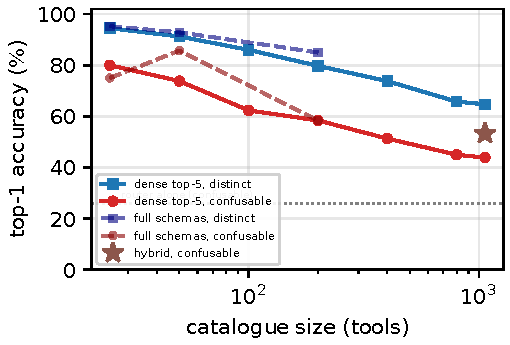
\includegraphics[width=0.95\columnwidth]{../figs/main_fig.pdf}
\caption{Top-1 selection accuracy versus catalogue size, split by
confusability. The confusable curve sits far below the distinct one at every
size, and full-schema prompting (dashed) does not close the gap. Dotted line:
the description-free router's confusable accuracy, flat in $N$ by
construction.}
\label{fig:retr}
\end{figure}

\subsection{Confusability moves the failure, it does not create it}
The cross-sectional gap is partly compositional: confusable queries belong to
large sibling families, over-represented at large $N$. For each of the 212
queries whose gold tool has confusers we therefore built two catalogues of the
\emph{same} size $N=200$ for the \emph{same} query: one excluding every
confuser, one with up to four forced in, displacing an equal number of random
distractors. Injecting confusers costs dense retrieval $-11.3 \pm 4.3$ points
of top-1 recall but only $-2.8 \pm 2.2$ of top-5 (95\,\% CIs over paired
differences); for BM25, $-2.8 \pm 2.6$ and $-1.9 \pm 1.8$.

This is a more useful result than a flat claim that retrieval breaks. Confusers
reliably displace the gold tool from rank~1, but rarely out of the top~5. In a
retrieve-then-select pipeline the gold tool therefore usually survives into the
candidate set, and the burden of telling \texttt{listServiceCatalog} from
\texttt{listResourceCatalog} is handed to whichever model does the final
selection. The question is whether that model can carry it.

\begin{table}[t]
\caption{Tool selection. C/D = confusable/distinct accuracy; res = outputs naming a real tool; $c_{\mathrm{sev}}$ = mean severity-weighted error cost over all predictions, charging an unresolvable name by the operation class it requests; dcall = queries ending in an unrequested \texttt{DELETE}.}
\label{tab:main}
\centering\scriptsize
\setlength{\tabcolsep}{3.2pt}
\resizebox{\columnwidth}{!}{%
\begin{tabular}{@{}lrrrrrrr@{}}
\toprule
Method & $N$ & Acc & C & D & res & $c_{\mathrm{sev}}$ & dcall \\
\midrule
Full schemas & 200 & 77.8 & 58.4 & 85.0 & 91 & 0.86 & 6.2 \\
BM25 top-5 & 1062 & 54.9 & 38.7 & 71.5 & 74 & 1.02 & 4.8 \\
Dense top-5 & 1062 & 54.2 & 43.9 & 64.7 & 87 & 1.66 & 10.5 \\
\; + PA-Tool rename & 1062 & 53.2 & 42.9 & 63.8 & 86 & 1.73 & 11.0 \\
No schemas (8B) & 1062 & 0.2 & 0.5 & 0.0 & 0 & 4.51 & 22.0 \\
Router 1.7B, untuned & -- & 0.0 & 0.0 & 0.0 & 0 & 6.78 & 27.0 \\
Router 1.7B, LoRA-1500 & -- & 30.8 & 25.9 & 35.7 & 43 & 3.02 & 22.0 \\
\textbf{Hybrid} (router $\cup$ dense-5) & 1062 & 62.3 & 53.3 & 71.5 & 93 & 1.43 & 9.8 \\
\bottomrule
\end{tabular}}
\end{table}

\subsection{The selector amplifies the penalty it inherits}
Table~\ref{tab:main} gives end-to-end selection. Retrieval into a five-tool
candidate set followed by the 8B selector reaches 54.2\,\% top-1 on the full
1,062-tool catalogue, against a top-5 recall ceiling of 61.1\,\%. The
interesting quantity is how much of that ceiling each subgroup converts.
Conditioned on the gold tool being present in the candidate set, the selector
picks it 95.7\,\% of the time for distinct tools but only 80.3\,\% of the time
for confusable ones. The confusable/distinct gap therefore \emph{grows} from
12.9 points at the retrieval stage to 20.8 points end-to-end: the selector does
not absorb the ambiguity that retrieval passes to it, it adds to it.

This is not an artefact of retrieval. With BM25 candidates the end-to-end gap
is 32.8 points (38.7 vs 71.5), tracking that retriever's larger recall gap;
and removing the candidate bottleneck entirely does not close it. At $N=200$, putting \emph{every} schema in
the prompt raises overall accuracy from 74.0\,\% to 77.8\,\%, but the entire
gain lands on distinct tools (79.7 $\rightarrow$ 85.0); accuracy on confusable
tools is identical to the decimal (58.4 vs 58.4), bought with 4,536 prompt
tokens instead of 211 and 22.8\,s per query instead of 1.1\,s. Twenty-one times the context bought no improvement where the problem is.
We do not claim the distinguishing information is absent from the schema text;
what we measure is that our selector did not exploit it, and that supplying
more of it did not help. Retrieval, usually framed as trading accuracy for
cost, gave up nothing on the confusable subset in our setup.

\subsection{Renaming does not transfer to a standardised catalogue}
PA-Tool-style renaming is the cheapest published remedy for small-model tool
errors~\cite{patool}, and on this catalogue it does not help: 53.2\,\% against
54.2\,\% for the same pipeline with native names, with the confusable subgroup
essentially unchanged (42.9 vs 43.9). The mechanism is visible in the
catalogue itself. Stripping the \texttt{TMFxxx} prefix and snake-casing the
operation makes 293 of 1,062 tools (27.6\,\%) share a name with at least
one other tool, because the standards code \emph{is} the disambiguator between
sibling APIs. Renaming either collides or must re-encode the same information as a domain
prefix, so in our setup pretraining-aligned naming had nothing left to add.

\subsection{Tool knowledge has to be trained in, and it is size-invariant}
In the description-free setting (no schemas in the prompt, roughly 90 tokens) the 8B reasoning model scores 0.2\,\% and the untuned 1.7B scores 0.0\,\%.
Neither can name a TM~Forum operation from pretraining. A LoRA adapter trained
only on template-generated request/tool pairs lifts the 1.7B to 30.8\,\% at
0.30\,s per query; a shorter 300-step run reaches 24.6\,\%, so the recipe is
not saturated at the budget we could afford. The comparison that matters is
not 30.8 against 54.2 but the shape of the curves (Fig.~\ref{fig:retr}):
the router never sees the catalogue, so its accuracy is constant in $N$ by
construction, while the retrieval pipeline falls from 93.8\,\% at $N=25$ to
54.2\,\% at $N=1062$. At full scale the router alone already matches dense
retrieval's top-1 recall (30.8 vs 32.5) without an index.

It is not, however, safe to let it act. Only 43\,\% of its outputs name an
operation that exists, and 22\,\% of queries end in a destructive call that
was not requested ($c_{\mathrm{sev}} = 3.02$, against 1.66 for retrieval).
A description-free router is a cheap \emph{proposer} of candidates and a bad
executor; the accuracy number alone hides this completely.

\subsection{The two signals are complementary}
The hybrid raises accuracy from 54.2\,\% to 62.3\,\% ($+8.1$ points) at the
full catalogue for three extra prompt tokens. The
gain is concentrated where the problem is: confusable accuracy rises from
43.9\,\% to 53.3\,\% ($+9.4$), and candidate recall from 61.1\,\% to
69.5\,\%. The router contributes candidates that retrieval misses rather than
reranking the ones it finds, and routing its proposal through a selector that
can see schemas also repairs its safety profile: the hybrid's $c_{\mathrm{sev}}$
is 1.43 and its dcall 9.8\,\%, both better than dense retrieval alone and far
better than the router acting by itself. A domain-tuned router earns its cost
as a \emph{recall} source at scale, not as a replacement selector; the weaker 300-step adapter already gave $+5.9$.

\subsection{What a wrong tool is, and how to price it}
Of the 192 errors the dense pipeline makes at $N=1062$, 138 name a real tool.
Among those, 77.5\,\% keep the correct verb and 93.5\,\% the correct severity
class, but only 18.1\,\% stay inside the correct API: \emph{right action,
wrong object} is the dominant failure mode. Severity almost never escalates,
so a ``did it escalate'' check reports a clean run; the damage is that 44 of
those 138 errors substitute one \texttt{DELETE} for another on a different
entity. We therefore report \emph{dcall}, the share of queries ending in a
destructive call the request did not ask for: 10.5\,\% for dense top-5.

Scoring this correctly matters. Charging unresolved outputs at read severity, the obvious default, makes the two 0\,\%-accuracy baselines the
safest-looking systems in the table. Once a model emitting
\texttt{TMF630\_\allowbreak removeWorkOrder} is charged for having asked for a deletion
whether or not that operation exists, the ordering inverts: $c_{\mathrm{sev}}$
is 6.78 for the untuned router and 4.51 for the schema-free 8B, against 1.66
for dense retrieval and 1.43 for the hybrid.

\smallskip\noindent\textbf{Arguments fail independently.} With the correct tool supplied, the selector names the right parameters almost always (key precision 94.6\,\%,
recall 98.7\,\%) but gets every value right in only 58.7\,\% of calls
(per-value exact match 77.3\,\%). Composed with selection at the full
catalogue, a complete correct call lands at roughly 32\,\%. Arguments are thus a failure source of comparable size to routing and largely
independent of it, so a single blended ``tool-call accuracy'' would misattribute
half the loss to the router.

\subsection{Abstention, and why accuracy is the wrong headline}
With the gold tool removed and \texttt{NONE} the only correct answer, the
pipeline abstains correctly 29.1\,\% of the time, naming a wrong tool in seven cases out of ten, at the highest severity cost we measured (2.74).
Abstention is worst where it matters: 21.7\,\% with confusers present against
36.7\,\% without. A sibling operation is close enough to look like an answer.
This mirrors the finding that replacing a router model with a retriever preserves
selection quality but cannot provide abstention~\cite{ondevice_routing}, on a
catalogue where close enough may be a \texttt{DELETE}.


\section{Discussion and Limitations}
\textbf{Renaming is not free here.} Stripping \texttt{TMFxxx} and snake-casing
the operation leaves 293 of 1,062 tools (27.6\,\%) sharing a name. We resolve
collisions with a domain token from the API title, which reintroduces what
renaming was meant to remove and still leaves five same-API collisions.

\textbf{Scoring severity is easy to get wrong.} Our first version of
$c_{\mathrm{sev}}$ charged unresolvable outputs at read severity, which ranked
the two 0\,\%-accuracy baselines as the safest systems we measured. Any
severity metric over free-form tool names has to price what the model
\emph{asked for}, not only what it successfully named.

\textbf{Limitations.} Queries are model-written from the specifications, which
if anything favours the retrievers; the confusability rule is a declared
lexical heuristic, not semantic ground truth; all models are laptop-scale, and
a frontier selector may discriminate better; and we evaluate single-call
selection only.




\section{Conclusion}
On this standardised telecom catalogue a major routing failure arises from
discrimination between sibling operations rather than candidate recall, and in
our experiments the gap is not resolved by schema renaming, a larger untuned
model, or additional schema context. A small domain-tuned router is complementary to retrieval, not a substitute. The results we would act on first are the safety ones: a router that names a
real operation 43\,\% of the time, and a pipeline that says ``none of these''
29\,\% of the time when nothing fits, are safety problems before they are
accuracy problems, in a domain where the closest-looking sibling may be a
\texttt{DELETE}\@.
Next: multi-step traces and a confirmation gate on deletions.


\balance
{\scriptsize
\bibliographystyle{IEEEtran}
\bibliography{refs}}
\end{document}
